%!TEX root = ../main.tex

\chapter{Measurements}
\label{ch:measurements}

This chapter evaluates the generated automaton. The measurements we performed focused on the capabilities of the \pru{} of the BeagleBone Black \sbc{}. The motivation of the measurements is to ensure the real-time capabilities of the device.

The guarantees most system can give are soft deadlines, meaning that the system provides best effort, but does not guarantee hard real-time guarantees. There are hard real-time operating systems like \textls{VxWorks} or \textls{FreeRTOS}.

The BeagleBone Black uses a 4.1.x \textls{RT}-Preempt patched kernel, which means it can serve hard real-time functions, but still the operating system and software running on them should be considered as non-reliable components. To bypass the operating system, one can use the \pru{}s embedded in the AM335x processor core.

In this chapter the automaton, and the PRU itself is measured. The measurement results depicted situations, where hard real-time requirement might fail because of missing a deadline.

\section{Test automata generation}

This section will describe the creation, and properties of the automata during the evaluation process.

We defined our test automata using the regular expression language introduced in \ref{sec:viatra_regex}. The \emph{AND} operator is the best way to create exponentially increasing automata with relatively small alphabet. An example for pattern declaration with regular expression is presented in \cref{lst:sample_regex}.
The compiler while minimizing the automata realize this pattern like a bit vector of events. The pattern given do not have any constraint for the order of events, therefore the completeness of the pattern can be imagined like a bit vector of length $n$, where $n$ is equal to the size of alphabet, formally $n=|\Sigma|$. The pattern is completed, when every element of the bit vector have value of $1$.
With every incoming event, the corresponding bit is toggled to $1$. If we have a bit vector of length $n$, and we would like to get all the permutation which results in a bit vector of $1$ values, we have $2^n$ different combination. Without minimization, the size of the automata would be $n \cdot (n-1) \cdot (n-2) \ldots $ which is equal to $n!$.

\begin{lstlisting}[
	float,
	caption={Sample pattern declaration with an alphabet size of 5},
	label=lst:sample_regex
]
alphabet = {A,B,C,D,E}
expression eventExpression = A & B & C & D & E
\end{lstlisting}

\section{Compiled code size}

The first measurement was to measure the code size of an automaton with alphabet size with respect to compiler optimization level. The measurements were taken by generating the test automata with the appropriate alphabet size. The messaging framework was not included in the code.

\subsection{Environment}
\begin{itemize}
	\item \emph{Compiler:} PRU C/C++ Compiler v2.1.2
\end{itemize}

\subsection{Results}

\begin{figure}
	\centering
	\caption{Code size in bytes with respect to compiler optimization levels, and alphabet size}
	\begin{tabular}{l c c c c c}
		\toprule
		& \multicolumn{5}{c}{Alphabet size} \\
		\cmidrule(r){2-6}
		& 3 & 4 & 5 & 6 & 7 \\
		\midrule
		\texttt{Ooff} & $768$ &		$1460$ &	$3060$ & 	$6704$ & 	N/A \\
		\texttt{O0}   & $652$ &		$1332$ &	$2916$ & 	$6548$ & 	N/A \\
		\texttt{O1}   & $376$ &		$636$ &		$1220$ & 	$2924$ & 	$6960$ \\
		\texttt{O2}   & $348$ &		$576$ &		$1096$ & 	$2548$ & 	$6332$ \\
		\texttt{O3}   & $336$ &		$564$ &		$1084$ & 	$2616$ & 	$6332$ \\
		\texttt{O4}   & $312$ &		$540$ &		$1060$ & 	$2592$ & 	$6308$  \\
		\bottomrule
	\end{tabular}
	\label{fig:code_size_table}
\end{figure}

\begin{figure}
	\centering
	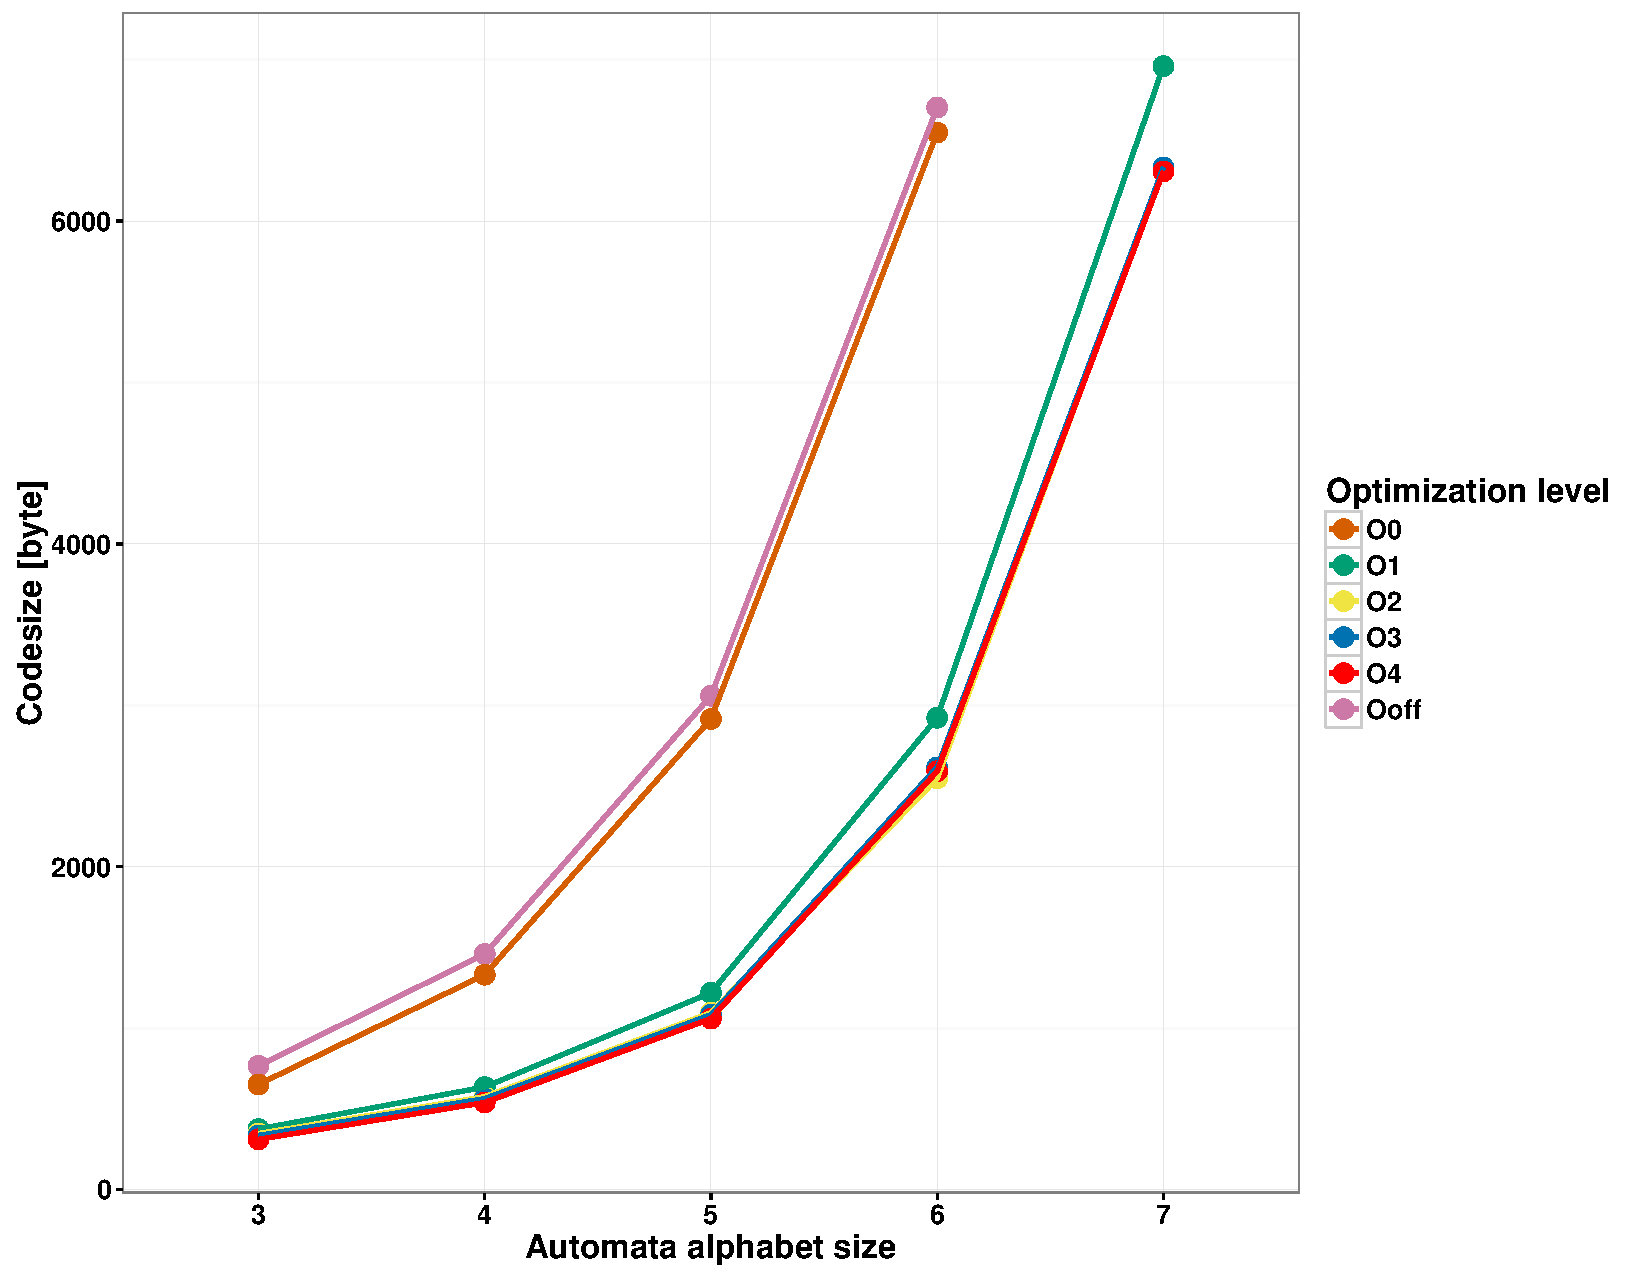
\includegraphics[width = \textwidth]{include/figures/code_size}
	\caption{Code sizes with respect to alphabet size and optimization level}
\label{fig:code_size}
\end{figure}

\subsection{Evaluation}

The \texttt{clpru} compiler have five stages of optimization levels. These levels describe the following behavior:
\begin{itemize}
\item \texttt{O0:} Optimizes register usage.
\item \texttt{O1:} Uses -O0 optimizations and optimizes locally.
\item \texttt{O2:} Uses -O1 optimizations and optimizes globally (default).
\item \texttt{O3:} Uses -O2 optimizations and optimizes the file.
\item \texttt{O4:} Uses -O3 optimizations and performs link-time optimization.
\item \texttt{Ooff:} Disables all optimization.
\end{itemize}

\cref{fig:code_size} depicts a plot of the data contained in \cref{fig:code_size_table}. The code size compiled with \texttt{Ooff} and \texttt{O0} options have minor difference, while both optimization level ran out of the \si{8}{kB} program memory at alphabet size of $7$.

The optimization level of \texttt{O1}, \texttt{O2}, and \texttt{O3} halves the code size, but there is no major code size reduction above \texttt{O1}. Level \texttt{O2}, \texttt{O3}, and \texttt{O4} generates practically the same code size.

The reason behind the huge reduction when O1 is enabled is that reduction of code size while utilizing optimization level \texttt{O1} caused by local optimization. The \emph{handleEvent} method of the automata have all the logic the execution needs, therefore the \texttt{O1} level can locally optimize this method. The program flow is very basic, meaning \texttt{O2}, and \texttt{O3} have minimal effect on code size, when it does global optimization of code.

\section{Message send time}

This measurement captures the performance of the \emph{rpmsg} framework, by benchmarking the time overhead with message sending to the \pru{}. This measurement is useful to determine how big the impact can be on an application, where the agent inside the application send the appropriate events down to the \pru{}.

\subsection{Environment}
\begin{itemize}
	\item \emph{Compiler:} PRU C/C++ Compiler v2.1.2
	\item \emph{Linux kernel version:} 4.1.24-ti-rt-r61
	\item \emph{g++ version:} 4.9.2
\end{itemize}

The measurement was done by a benchmarking application written in \cpp{} (\cref{lst:benchmark_code}). The application send a character '1', and a newline character to the \pru{} through the virtual device. The code was compiled explicitly with the \texttt{-O0} argument, to disable optimizations of any kind. The \emph{for} cycle use a modulo based indexing. This is needed because after the warm up period, the same code will be executed, ensuring the code is cached inside the processor, and branch prediction will not be an issue.


\begin{lstlisting}[
	float,
	caption={The benchmark code used in the measurement},
	label=lst:benchmark_code,
	language={C++}
]
#include <unistd.h>
#include <fcntl.h>
#include <sys/types.h>

#include <iostream>
#include <fstream>
#include <chrono>
#include <thread>

#define N 10
#define BUFFER_SIZE 10000

int main(int argc, const char * argv[]) {
	std::chrono::high_resolution_clock::time_point startBuffer[BUFFER_SIZE];

	int file = open("/dev/rpmsg_pru30", O_WRONLY);
	char msg[] = {
		'1', '\n'
	};

	for (int i = 0; i < N * BUFFER_SIZE; ++i) {
		startBuffer[i % BUFFER_SIZE] = std::chrono::high_resolution_clock::now();
		write(file, msg, sizeof(msg));
	}
	close(file);

	std::ofstream output;
	output.open("benchmark-result.csv");
	output << "delta" << std::endl;
	for (int i = 0; i < BUFFER_SIZE-1; ++i) {
		auto value =
			std::chrono::duration_cast<std::chrono::nanoseconds>(
				startBuffer[i+1] - startBuffer[i]
			);
		std::cout << value.count() << std::endl;
	}
}
\end{lstlisting}

\subsection{Results}

The measurement contains 3 datasets.
\begin{itemize}
	\item \emph{Measurement 1:} With $1000000$ messages, interrupt based receiving on the \pru{} side.
	\item \emph{Measurement 2:} With $10000$ messages, interrupt based receiving on the \pru{} side.
	\item \emph{Measurement 3:} With $10000$ messages, polling based receiving on the \pru{} side.
\end{itemize}

\begin{figure}
	\centering
	\caption{Measurement statistics in \si{\mics}}
	\begin{tabular}{l c c c}
		\toprule
		& Min & Median & Max \\
		\midrule
		Measurement 1 & 1.375 & 1.375 & 110.375 \\
		Measurement 2 & 1.791 & 1.833 & 135.708 \\
		Measurement 3 & 41.17 & 42.33 & 126.92 \\
		\bottomrule
	\end{tabular}
\end{figure}

\begin{figure}[h]
	\centering
	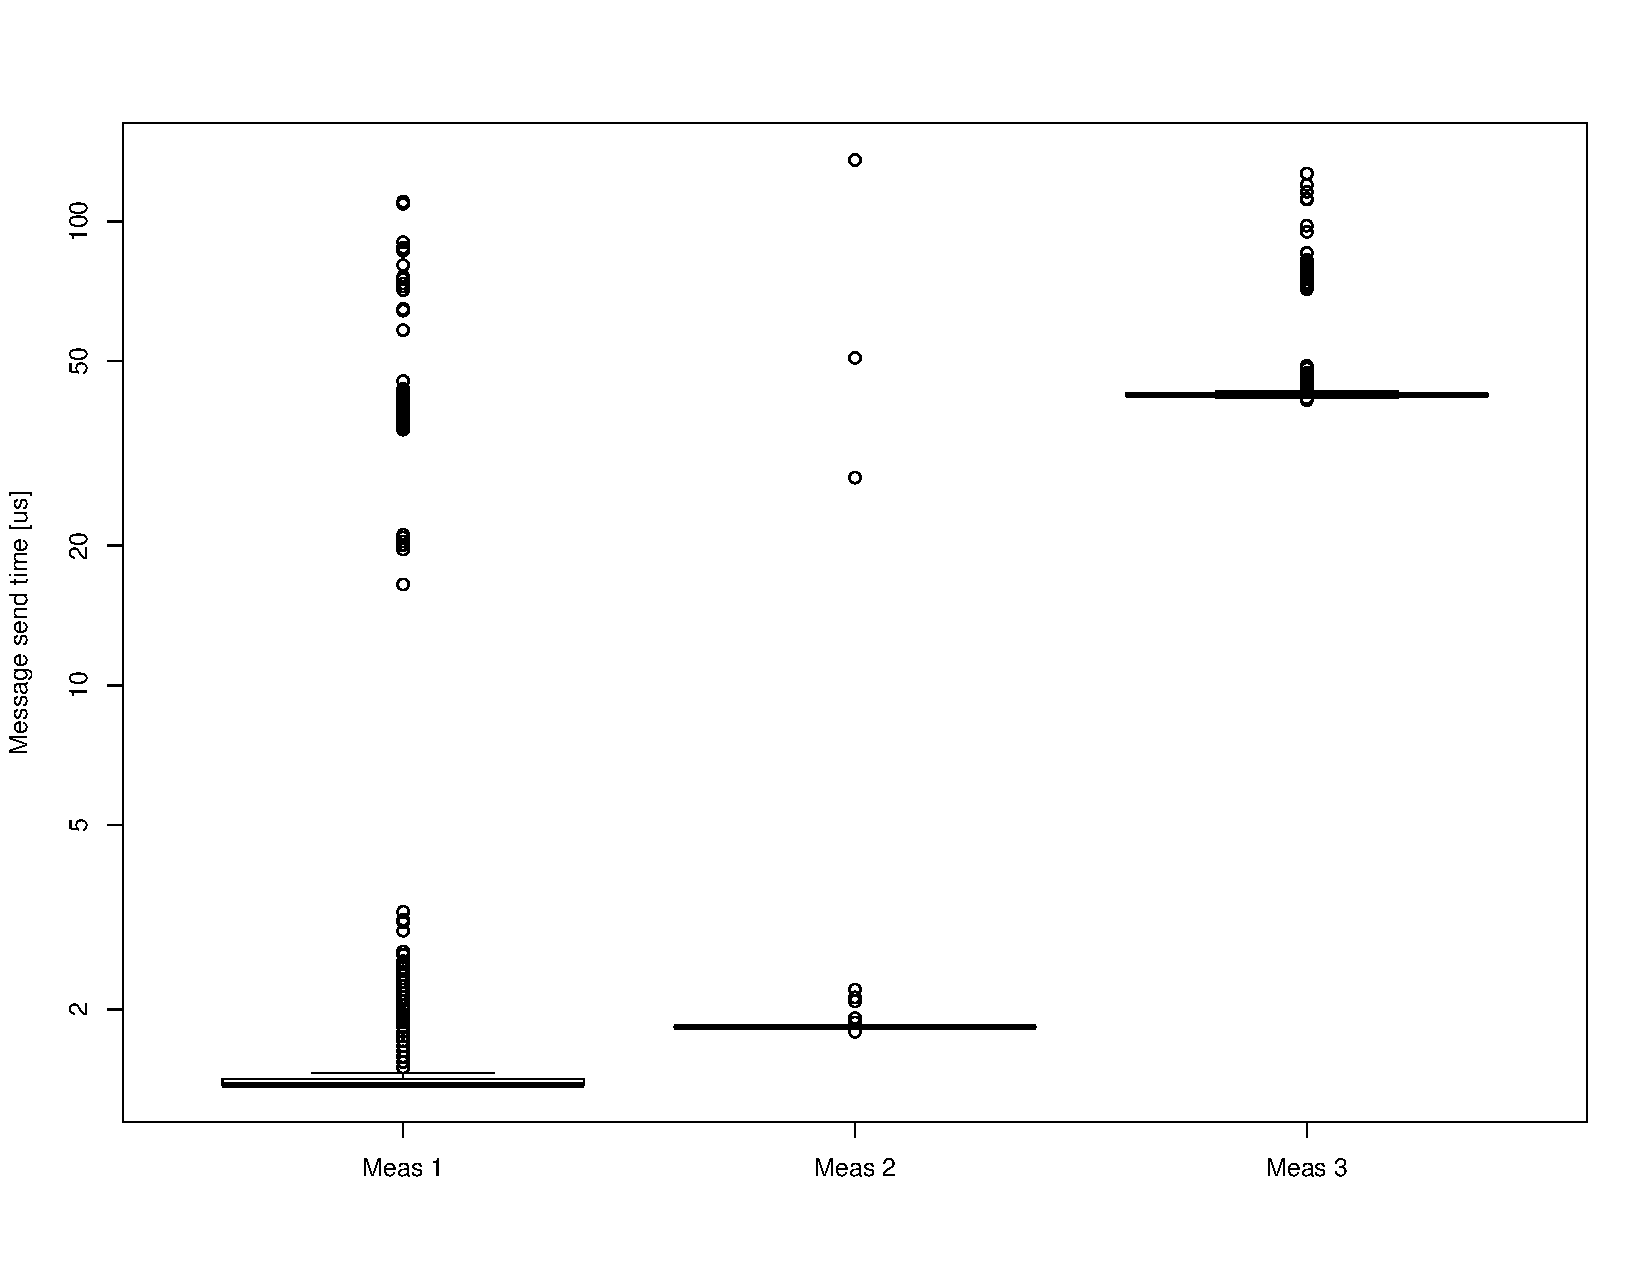
\includegraphics[width = \textwidth]{include/figures/rpmsg_boxplot}
	\caption{Boxplot of the measured data with logarithmic scale}
\label{fig:rpmsg_boxplot}
\end{figure}

\subsection{Evaluation}

The measurement uncovered some interesting properties, which can be traced back to the operating system. Generally all measurements have their median value very close to the minimal value. This means the most of the time, the sending time was consistent. The outliers mark the context switches of the operating system. The biggest time between messages in the measurement was \si{135}{\mics}. This means if the automaton have a millisecond based timing, lag caused by context switching should not be an issue. Note that the system was running this task only, therefore if other tasks are running with high resource needs, this value might increase.

Measurement 2 is a smaller dataset than measurement 1, the only change done was to the \texttt{BUFFER\_SIZE} definition. After taking the measurements again with the same result in the median, the final conclusion was found. The Linux kernel is doing clock scaling to save energy. The kernel have a discrete set of frequencies (\si{300}{\MHz}, \si{600}{\MHz}, \si{720}{\MHz}, \si{800}{\MHz}, \si{1000}{\MHz}), and before execution, the system is idle, therefore the kernel scales the \cpu{} back to \si{300}{\MHz}. When the benchmarking run with a small sample, the warmup loops get executed faster than the reaction time of the operating system resulting in a bigger overhead.

Measurement 3 shows the performance of a communication, where the \pru{} using poll based message receiving. This means the \pru{} will access the \textls{DDR3} memory trough the \textls{L3} interconnection bus which has non-deterministic behavior. The latency of the bus, and memory might vary with the system load.
The interrupt based solution have an interrupt flag, which can be set from the host processor. In the code, this interrupt flag prevents the unnecessary checks to the \textls{DDR3} memory, increasing the performance by approximately a factor of 50.

This measurement motivated to test the effect of different \cpu{} clocks further. The results are presented in \cref{sec:freq}

\section{Message send time as function of \cpu{} frequency}
\label{sec:freq}

\subsection{Environment}
\begin{itemize}
	\item \emph{Compiler:} PRU C/C++ Compiler v2.1.2
	\item \emph{Linux kernel version:} 4.1.24-ti-rt-r61
	\item \emph{g++ version:} 4.9.2
\end{itemize}

\subsection{Results}

\begin{figure}
	\centering
	\caption{Statistics of message overhead on differency \cpu{} frequencies in \si{\mics}}
	\begin{tabular}{l c c c}
		\toprule
		Freq & Min & Median & Max \\
		\midrule
		\si{300}{\MHz}  & 137.0 & 223.7 & 2335.0 \\
		\si{600}{\MHz}  & 66.21 & 68.33 & 249.92 \\
		\si{720}{\MHz}  & 56.08 & 57.38 & 172.08 \\
		\si{800}{\MHz}  & 50.92 & 51.96 & 143.58 \\
		\si{1000}{\MHz} & 41.54 & 42.38 & 118.62 \\
		\bottomrule
	\end{tabular}
\label{fig:rpmsg_freq_stats}
\end{figure}

\begin{figure}[h]
	\centering
	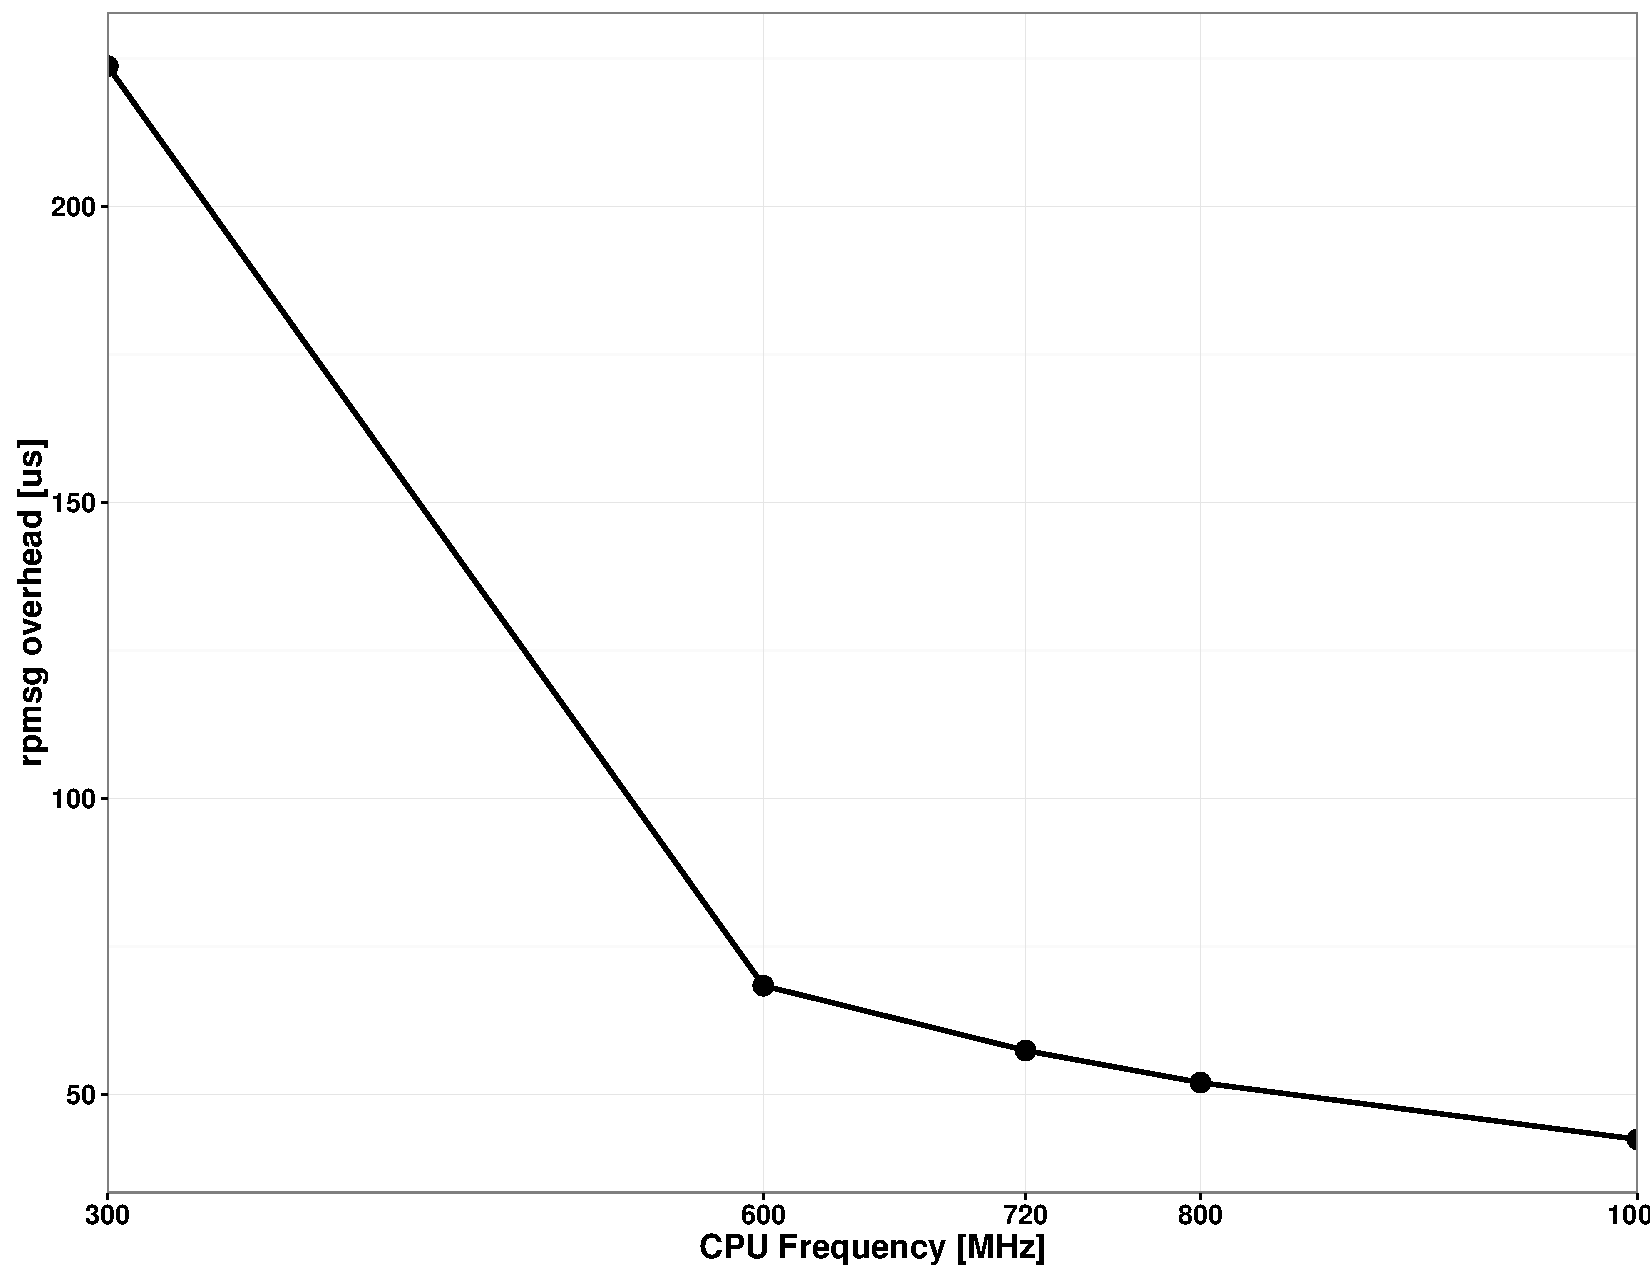
\includegraphics[width = \textwidth]{include/figures/rpmsg_freq}
	\caption{Median of rpmsg framework overhead with regards to \cpu{} frequency}
\label{fig:rpmsg_overhead_plot}
\end{figure}

\subsection{Evaluation}

Starting from 600MHz, the decrease in the overhead is proportional to the frequency of the \cpu{}, but interestingly \si{300}{\MHz} shows a bigger increase in the execution time of message sending. Another interesting value showing this discrepancy is the maximal time difference at \si{300}{\MHz} (\cref{fig:rpmsg_freq_stats}). Currently we are unable to explain the reason of this anomaly.

\section{Event execution time}

The \emph{switch-case} control structure when the compiler can optimize is implemented as a lookup table (\emph{LUT}). The big advantage of a lookup table is it have a constant worst-case complexity of selecting the correct branch. Another realization is the \emph{if-else} structure, where the switch is implemented as a series of branches. To find out which is implemented when the automata compiled, we need to decompile the code. The \pru{} \textls{SDK} provides the \texttt{disas} utility, which can disassemble the compiled code.

When inspecting the code, the control structure in \cref{lst:disassembly} can be found. The \texttt{QE} in instructions \texttt{QBNE}, \texttt{QBLT} means \emph{Quick Branch} where the last part:
\begin{itemize}
	\item \texttt{NE}: Not equal
	\item \texttt{LT}: Less than
\end{itemize}

Therefore if one analyses the code, it's representing an \texttt{if-else} structure, meaning it iteratively compares the switch variable agains all case branches, and if it's matching, the program jumps to the appropriate branches code. The problem with this approach compared to the \emph{LUT} is the variable execution time, which is depending on the switches input variable.

In the case of the compiled automata, there might be execution time deviations between different branch executions. To measure this deviation, the code was modified. For every measurement, the branch serving out the appropriate event was instrumented with an assignment to one of the \gpio{} pins. The width of the pulse defines the execution time of the automata.

\begin{lstlisting}[
	float,
	caption={Part of the disassembly of the \emph{handleEvent} method},
	label=lst:disassembly,
]
00000058     6900e002      QBNE 0x8, R0, 0
0000005c     21058500      JMP $C$L71
00000060     6901e002      QBNE 0x8, R0, 1
00000064     21043400      JMP $C$L30
00000068     0502e0e1      SUB R1, R0, 2
0000006c     4901e102      QBLT 0x8, R1, 1
00000070     21058500      JMP $C$L71
00000074     6904e002      QBNE 0x8, R0, 4
00000078     21060100      JMP $C$L132
0000007c     0505e0e1      SUB R1, R0, 5
00000080     4902e102      QBLT 0x8, R1, 2
00000084     21058500      JMP $C$L71
00000088     6908e002      QBNE 0x8, R0, 8
0000008c     21036700      JMP $C$L19
\end{lstlisting}


\subsection{Environment}
\begin{itemize}
	\item \emph{Compiler:} PRU C/C++ Compiler v2.1.2
	\item \emph{Linux kernel version:} 4.1.24-ti-rt-r61
	\item \emph{g++ version:} 4.9.2
	\item HAMEG HM1005 oscilloscope
\end{itemize}

\subsection{Results}

\begin{figure}
	\centering
	\caption{Statistics of message overhead on differency \cpu{} frequencies in \si{\mics}}
	\begin{tabular}{l c c c}
		\toprule
		Event & Measured div & Time base & Elapsed time \\
		\midrule
		A & 3.8 & 0.2 & 0.76 \\
		B & 3.8 & 0.2 & 0.76 \\
		C & 3.8 & 0.2 & 0.76 \\
		D & 3.8 & 0.2 & 0.76 \\
		E & 3.8 & 0.2 & 0.76 \\
		F & 3.8 & 0.2 & 0.76 \\
		G & 3.8 & 0.2 & 0.76 \\
		\bottomrule
	\end{tabular}
\label{fig:rpmsg_exec_stats}
\end{figure}

\subsection{Evaluation}

Because we know the assembly struct, a harsh estimation can be constructed to validate the results. The states of the test automata have transitions with all of the input events, therefore the number of transition outgoing from every transition is $2^7=128$. The control flow of a branch consists of 2 instructions. An instruction takes \si{5}{\ns}, therefore the approximated time to execute the automaton is $128 \cdot \si{5}{ns} = \si{640}{\ns} = 0.6\mics$. This is a rough estimate of the execution time, because it does not include additional instructions and calls, but the measured data in \cref{fig:rpmsg_exec_stats} is close to the value estimated.

\section{Conclusion}

These measurements uncovered how many hidden factors affect the response, and performance of a system. The preemptive behavior of the operating system plays an important role, but frequency governors may induce jitter in the latency of the communication.

Apart from host side performance, the poll based communication illustrates how big is the time penalty of a \textls{DDR3} memory access. The test automation used in the measurements was the biggest which could be fitted inside the \pru{} instruction memory with $7 \cdot 2^7 = 896$ transitions total, $128$ transition possibility per event. The stepping of the automaton was handled under \si{1}{\mics}, therefore the automaton limited much by size of the automaton rather then the execution time of it.
